% Opening material before first \section

%%%%%%%%%%%%%%%%%%%%%%%%%%%%%%%%%%%%%%%%%%%%%%%%%%%%%%%%%%%%%%%%%%%%%%%%%%%%%%%%%%%%%%%%%%%%%%%%%%%%%%%%%%%5





The basic model of viral replication was developed in the early 1990s during research into the functioning of HIV within the body. It assumes a constant release of infectious particles from infected cells. The model is deterministic, contained in a set of three ODEs, but is consistent with an underlying stochastic model as the expected process behaviour. In this underlying model, each infected cell releases virions according to a poisson process.\par 

Despite being quite effective, this assumption is only an approximation of reality and is non-cognisant of what happens within cells. It's wide speard use in the BMVR may have even wrongly painted our understanding of how viral release really takes place. In reality, the rate of viral release will not be at its full capacity at the moment of innoculation. Some models have addressed this by incorporating an ``ecclips phase'' during which the cell is non-productive. It also seems possible that the intracellular load of an infected cell could have something to do with its production rate. This will of course differ between viruses and intracellular bacterial infections, and even between species of each.  \par
A barrier to understanding viral release in particular is that viruses are incredibly small and are not easily observed, as is generally  (just about)  possible for bacteria. Despite this difficulty, a group at Los Alomos has recently published work attempting to quantify exactly this: the number of HIV particles produced by single infected cells over time. What they found was that the release behaviour is not at all constant, but stochastic and intermittent. Large packets of varing size are released in apparent bursts, at times intervened by relative inactivity.\par
This chapter explores the fundamental differences between two extremes of the viralaty strategy space: constant ``budding'' release, and ``all at once'' burst release. And a couple of mathematically framed hypotheses are presented which explain potential advanteges to so called bursting and intermittent virality.


\begin{itemize}

\item \textbf{Other work and lack of ``additional effects''}
Comparing bursting and budding virality is not our idea. There is a niche of prexisting literature which does include stochasic models of each regime and the relative differences seen in analysis. This section overviews some of the work that has previously been done in the area, and identifies only a limited consideration for ``additional effects''. That is, factors significant to overall viral success that go beyond merely the microscopic replication rate within cells, and the release behaviour. Namely, depleatable toxic granules within cells, and locally finite immuno factors in the extracellular medium. My work over the following sections proposes additional mathematical quantifications to what has been termed by ``(inserty name)'' as the advantage of ``flooding''. Or how in a burst style release, there is higher likelihood of using up the local capacity of the host's immune system.   \cite{williams2021stochastic}
\cite{williams2024reproduction}
\cite{carruthers2020stochastic}
\cite{gillard2014modeling}
\cite{garoff1998virus}
\cite{golovliov2003attenuated}
\cite{jones2012subversion}
\cite{cowley2011immunity}
\cite{ribeiro2002vdt}
\cite{ribeiro2010estimation}
\cite{deboer2012our}
\cite{perelson1999mathematical}
\cite{perelson1996hiv}
\cite{bird2015escape}
\cite{bird2015nonlytic}
\cite{perelson2018introduction}
\cite{wood2014dose}
\cite{ciupe2017host}
\cite{conway2018modeling}
\cite{komarova2007viral}
\cite{anderson1988role}
\cite{beauchemin2011review}
\cite{rong2013analysis}
\cite{guedj2013modeling}
\cite{nelson2004age}
\cite{brown2006intracellular}
\cite{kitagawa2018pde}
\cite{conway2018modeling}
\cite{di2008note}
\cite{stirzaker2006processes}
\cite{capistran2018extracellular}
\cite{ciupe2024incorporating}
\cite{brockwell1986extinction}.




\item \textbf{Replicator suppressor}

Over the handful of lucocyte types known to science, most contain packets of toxic material called granuoles (of course, not least, granuolocytes). These generally oxidative substances are employed by the immune cells to attack invading pathogens. The leucocytes of interest in our resreach, macrophages and neutrophils, both contain granuoles. Neutrophils contain more and use them slightly differently, lysing themselves to release the inflamatory packats to the extracellular medium. Whereas macrophages employ the toxic granuoles intracellularly, merging the bags of toxin with phagosomal membranes which harbour pathogen after engulfing has taken place. I believe Neutrophils dothis as well in addition to the lyse method. And it is this dynamic which forms the basis of the model presented here.\par
Basically, picture a leukocyte which has just engulfed some number of pathogen. It also contains a count of toxin containing granules which are assumed to be depleated in the process of being used to kill pathogen. With the model specification as given, it can be shown that the number of incident pathogen has a substantial effect of the survival potential of the infection.   




\item \textbf{N = 2 results}

We were interested in describing an infection across multiple containing cells. For this aim, we began to consider the simple case of an infection going from one cell to another. A birth death catastrophe process in the first which once completed leads to the instantiation of a second BDC process. It's as if all of the bacteria were to go from one cell to the next immediately. There are four quantities of this model: the burst time and size in both the first and second process; $t_1$, $r_1$ \& $t_2$, $r_2$. The first two of these can be found in distribution using content of chapter 2. The second burst quantities are more challenging, but we have made progress in finding their distributions.\par
Though this part of the work didn't lead to a grand new model for describing multi-intracellular infection dynamics, it did in part inspire the content of the next section, which takes the concept of successive rounds of a BDC process and incorporates an additional effect.  







\end{itemize}








\begin{figure}[H]
    \centering
    % First row of two figures
    \begin{subfigure}{0.48\textwidth}
        \centering
        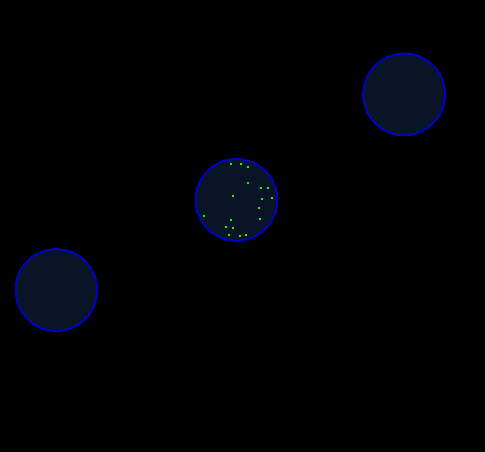
\includegraphics[width=\textwidth]{figures/IMG_ch7/Bursting/Basic/basic1} % Adjust the image path as necessary
        \caption{}
        \label{fig:figure1}
    \end{subfigure}
    \hspace{\fill} % Optional: adds space between figures
    \begin{subfigure}{0.48\textwidth}
        \centering
        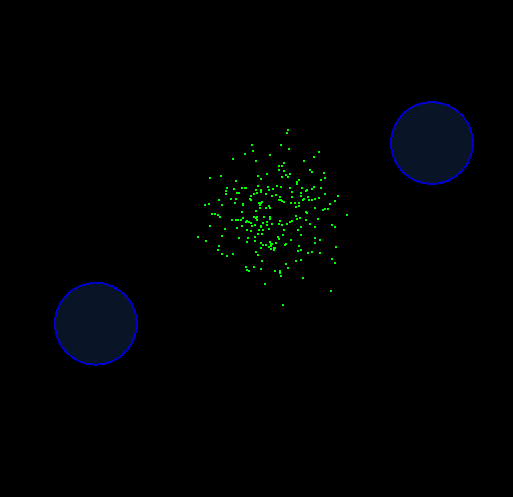
\includegraphics[width=\textwidth]{figures/IMG_ch7/Bursting/Basic/basic2} % Adjust the image path as necessary
        \caption{}
        \label{fig:figure2}
    \end{subfigure}

    \vspace{1em} % Small vertical space between rows

    % Second row of two figures
    \begin{subfigure}{0.48\textwidth}
        \centering
        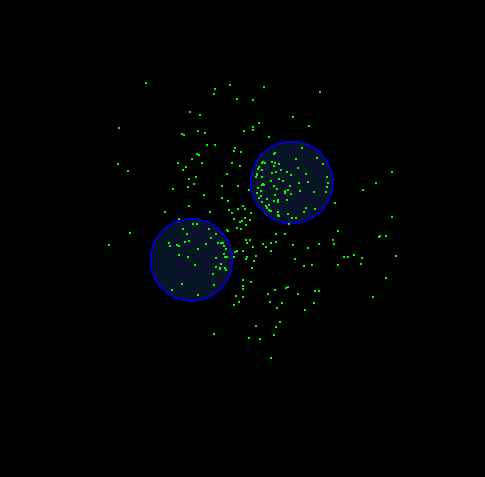
\includegraphics[width=\textwidth]{figures/IMG_ch7/Bursting/Basic/basic3} % Adjust the image path as necessary
        \caption{}
        \label{fig:figure3}
    \end{subfigure}
    \hspace{\fill} % Optional: adds space between figures
    \begin{subfigure}{0.48\textwidth}
        \centering
        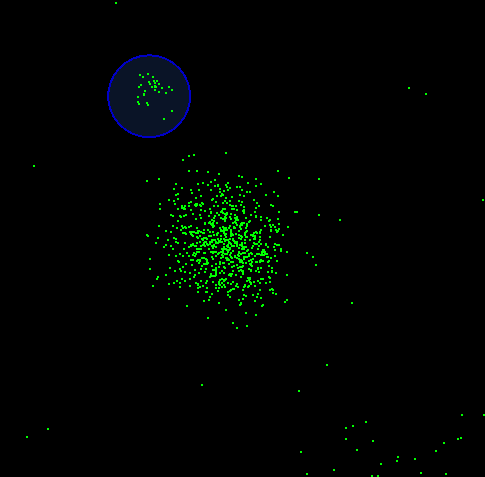
\includegraphics[width=\textwidth]{figures/IMG_ch7/Bursting/Basic/basic4} % Adjust the image path as necessary
        \caption{}
        \label{fig:figure4}
    \end{subfigure}

    \caption{(a), Intracellular replication before bursting. (b) Cell bursts, and the contents spans the extracellular space before finding new hosts.  (c) Macrophages are motile. They wander around the extracellular matrix,  phagocytosing debris and extracellular pathogens alike.  (d) A second round of cell bursting is displayed, in this case, the second load is larger.}
    \label{fig:four_figures}
\end{figure}















\subsection*{Three non-basic modifications}
Here we shall seek to describe rigorously the non-extinction probabilities though time of processes with varied initial state that are subject to non-linear dynamics. Basically, a number of replicative units found an infection within a host cell, their dynamics accord with a continuous-time birth death process. What is the probability at time $t$ there is at least one unit still alive, i.e. ``the infection'' has not died out? This will depend on the criticality of the process --- whether a given unit is expected to leave behind greater or less than a replacement of itself --- which will depend on the birth and death rates, $\lambda$ and $\mu$. But we are here interested in the effect of process non-linearities, and what implications these have for survivability at varied initial counts, $\xx_0 = n$.\par

Taking the standard birth-death process, $\xt$, for now with one initial replicative unit, $\xx_0$. Its transition rates are defined
\begin{align*}
\pr{\Delta \xt = 1} &= \lambda \xt \delt + o(\delt),\\
\pr{\Delta \xt = -1} &= \mu \xt \delt + o(\delt),\\
\pr{\Delta \xt = 0} &= 1 - (\lambda + \mu) \xt \delt + o(\delt),
\end{align*}
(with $\Delta \xt = \xdt - \xt$). In this linear-format, the process is said to be critical exactly when $\lambda = \mu$. Each replicative unit eventually dies or divides, so when chances for each of these eventualities balances, the expected number of ``offspring'' for a given unit will be 1. More rigorously, defining the count of progeny units left behind as $Z$:
\begin{align*}
\pr{Z=2} &= \frac{\lambda}{\lambda + \mu}\\
\pr{Z=0} &= \frac{\mu}{\lambda + \mu}
\end{align*}
Left behind should be read as ``following the next event'', so time become irrelevant. When $\lambda = \mu$, 
$$\pr{Z=2} = \pr{Z=0} = \frac{\lambda}{2\lambda} = \frac{1}{2}.$$
And the expected replacement count for a particles is 1;
$$\mean{Z} = 0\cdot \pr{Z = 0} + 2 \cdot \pr{Z = 2} = 2\cdot \frac{1}{2} = 1.$$
If $\lambda > \mu$, this value is greater than 1, and if $\lambda < \mu$, it's less than 1, these cases are termed supercritical and subcritical respectively.
\vspace{15pt}
\begin{adjustwidth}{2cm}{}
\begin{itemize}
\item[$\mean{Z} > 1$:] \textbf{Supercritical}. Given on-average replacement and increase, a population may avoid extinction indefinitely. This occurring with some probability $S(t)$ as defined below. 
\item[$\mean{Z} = 1:$] \textbf{Critical}. Despite each unit fully replacing itself in expectation, a critical birth death chain will inevitably decline to nothing. Interestingly, the expected time until this happens is infinite. 
\item[$\mean{Z} < 1:$] \textbf{Subcritical}. On average, each unit will not replace itself and the process will decline, though stochastically, with ultimate demise --- fixation at 0.
\end{itemize}
\end{adjustwidth}



\subsection{Gompertz Poisson first jump and expected value}
The Poisson process, as $\xt$ is defined
\begin{align*}
\pr{\Delta \xt = 1} &= \lambda \delt + o(\delt),\\
\pr{\Delta \xt = 0} &= 1 - \lambda  \delt + o(\delt);
\end{align*}
a constant rate of stochastic incidence events. 
\subsubsection{First jump probability}
Defining $\pr{\xt = i} = p_i(t)$, the move from state 0 to 1 can be quantified with the state zero probability, $p_0(t)$. And this can be computed in the following way. 
$$p_0(t+\delt) = p_0(t)[1 - \lambda \delt + o(t)].$$
In plain English: the probability $\xdt = 0$ is the likelihood $\xt = 0$, and, in the interval $(t, t + \delt]$, nothing happens. There is no ``immigration'' event. When taken in the limit $\delt\to 0$, this formula derives the ODE, 
$$\frac{p_0(t+\delt) - p_0(t)}{\delt} = \lambda p_0(t)+  o(\delt)$$
$$ \xrightarrow{\underset{\delt \to 0}{}}  \hspace{5pt}  \ddt{p_0(t)} = \lambda p_0(t).$$ 

\noindent
This is simple, of course. And the solution is a basic decaying exponential, $p_0(t) = \ee^{-\lambda t}$. But what would happen if we modified the addition rate, making the process inhomogeneous in time. Say for example the rate itself was a decaying exponential: $\lambda \to \lambda(t) = \ee^{-t}$?  
\begin{align*}
\pr{\Delta \xt = 1} &= \lambda(t) \delt + o(\delt),\\
\pr{\Delta \xt = 0} &= 1 - \lambda(t)  \delt + o(\delt);
\end{align*}
The question is: can we make the same simple derivation of $p_0(t)$ without issue? It's not obvious at first that  everything will work out. When writing the first step equation,
$$p_0(t+\delt) = p_0(t)[1 - \lambda(\mathbf{?}) \delt + o(t)],$$
there is some ambiguity about what should be in the argument of $\lambda(t)$. Do we take the value at the start, or the end of the interval: $\lambda(t)$ or $\lambda(t+\delt)$? The probability that an event happens or not during the interval can not simply be defined by either of these. But in all likelihood, we are confusing ourselves for no reason. Because the equation is ultimately evaluated in the limit, it shouldn't matter. $\lim_{\delt\to0}(t+\delt) = t $, so the two cases end up being identical. It seems obvious when put like this, I just hesitate because things aren't always as they seem in probability theory and we wouldn't want to be caught out. In any case, it is possible and straightforward to verify the subsequent result.\par
With the inhomogeneous version of the equation,
$$\ddt{p_0(t)} = \lambda(t)p_0(t), \hspace{10pt} \lambda(t) = \ee^{-\alpha t},$$
$p_0(t)$ can be computed as
$$p_0(t) = \ee^{\lrb{\ee^{- t} - 1}  }$$  
With $\lambda(t) = \beta \ee^{-\alpha t}$, this generalises to
$$p_0(t) = \ee^{\frac{\beta}{\alpha} \lrb{\ee^{-\alpha t} - 1}  }.$$ 





\def\eval{0.36787}

\begin{figure}[h]
	
    \centering
    \resizebox{0.8\textwidth}{!}{%
    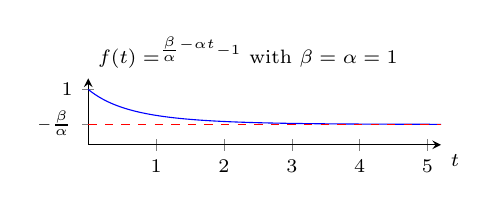
\begin{tikzpicture}
        \begin{axis}[
            xlabel={$t$},
            ylabel={$f(t) = \ee^{\frac{\beta}{\alpha}\lrb{\ee^{-\alpha t}} - 1  }$ with $\beta = \alpha = 1$ },
            axis lines=middle,
            xmin=0, xmax=5.2,
            ymin=0, ymax=1.2,
            width=0.5\textwidth,
            height=0.2\textwidth,
            xtick={0,1,2,3,4,5},
            ytick={0, \eval,1},
            yticklabels={0,$\ee^{-\frac{\beta}{\alpha}}$,1},
            tick label style={font=\scriptsize},
            xlabel style={at={(ticklabel* cs:1)}, anchor=north west, font=\scriptsize},
            ylabel style={at={(ticklabel* cs:1)}, anchor=south west, font=\scriptsize},
            legend style={at={(0.5,1.03)},anchor=south,legend cell align=left,font=\scriptsize},
            ]
            \addplot[blue, domain=0:5.2, samples=100] {exp(exp(-x) - 1)};
            \draw[red, dashed] (axis cs:0,0.367879) -- (axis cs:5.2,0.367879);
        \end{axis}
    \end{tikzpicture}
    }
    \caption{Decaying exponential function $f(t) = e^{{e^{-t}-1}}$.}
    \label{fig:exponential}
\end{figure}



\subsection*{Poisson Gompertz}

\begin{align*}
\pr{\Delta \xt = 1} &= \lambda(t) \delt + o(\delt),\\
\pr{\Delta \xt = 0} &= 1 - \lambda(t)  \delt + o(\delt);
\end{align*}



\subsubsection*{No added constant}

$\lambda(t) = \beta \ee^{-\alpha t}$
$$\mean{\xt} = \frac{\beta}{\alpha} \lrb{1 - \ee^{-\alpha t}}$$
$$p_0(t) = \ee^{\frac{\beta}{\alpha} \lrb{\ee^{-\alpha t} - 1}  }.$$ 


\subsubsection*{Added constant}

$\lambda(t) = \beta \ee^{-\alpha t} + \gamma$


$$\mean{\xt} = \frac{\beta}{\alpha} \lrb{1 - \ee^{-\alpha t}} + \gamma t$$



\subsection*{Deterministic version}

Considering a single unit exhibiting Gompertz activation.\par

\vspace{5pt}

\noindent
$N(t)$: activation of a node.
$$\ddt{N(t)} = \lrb{\lambda(t) - \mu} N(t)$$
\begin{itemize}
\item Gompertz growth rate: $\lambda(t) = \beta \ee^{-\alpha t} + \gamma$. Made up of,
\begin{itemize}
\item $\beta \ee^{-\alpha t}$: decaying term represents the reduced proliferation in response to recognition and desired ceasing, and
\item $\gamma$: constant, a sort of base-line growth rate. 
\end{itemize}
\item $\mu$: decline rate.
\end{itemize}
Formula: 
$$N(t) = N_0 \ee^{\lrbs{\frac{\beta}{\alpha} \lrb{1 - \ee^{-\alpha t} } + (\gamma - \mu) t }  }$$
Interesting case: When $\mu > \gamma$ and $\mu < \gamma + \beta \ee^{-\alpha t}$ when t = 0. Sufficient to say $\gamma < \mu < \gamma + \beta$.











































%%%%%%%%%%%%%%%%%%%%%%%%%%%%%%%%%%%%%%%%%%%%%%%%%%%%%%%%%%%%%%%%%%%%%%%%%%%%%%%%%%%%%%%%%%%%%%%%%%%%%%%%%%%5
